\section{Bump Map}

Jim Blinn在1978的\text{Simulation of Wrinkled surfaces}论文中使用一种灰度高度图来建模物体表面法线的扰动,扰动法向量的大小用
某些表面参数的偏微分和高度图来计算。要把扰动的法向量加入光照模型中进行计算,就必须是像素级的shading(因为顶点级的Gouraud shading
是逐顶点计算光照公式,最后每个像素都是这些顶点插值出来的,OpenGL的标准光照是基于Phong光照模型但使用Gouraud shading,Phong shading
是指插值顶点法向量在fragment基本计算光照公式)。

Bump Map是Phong Shading的一项扩展,表面法线用来计算顶点的光亮,它必须通过顶点插值来确定,虽然每个fragment都有一个独特的法线,
但法线不能准确表示表面的粗糙程度,而Bump Map就是为了影响法线的改变,最终影响颜色值,所以算是一种负责光方向的纹理映射,
不同的凹凸数据,使用不同的方法来影响法线,常见的有两种模式:
\begin{itemize}
    \item \text{Emboss Bump Map浮雕,使用HeightMap,用在diffuse lighting中}
    \item \text{Environment-mapped,使用grayscale height map}
    \item \text{DOT3 Bumap Map点乘凸凹贴图,使用NormalMap}
\end{itemize}

凹凸贴图通常保存为RGB纹理,纹理每个通道分别存储标准化方向向量的x、y、z轴的值,作为颜色数据,可以像其他的纹理一样,
进行采样插值,不管凹凸贴图分辨率大小,都会存在插值并对每个fragment法线产生作用

\subsection{Height Map}
高度图是存储高度信息的数据,通常计算XY方向上的倾斜度
\begin{gather*}
    x_gradient = pixel(x-1,y) - pixel(x+1,y) \\
    y_gradient = pixel(x,y-1) - pixel(x,y+1) \\
    normalNew = normal + (U * x_gradient) + (V * y_gradient)
\end{gather*}
在的Bump Map\cite{CGPP3ed}中,有一个公式更加通用
\begin{align*}
    n^{'} = S(n + rt_{1} + gt_{2})
\end{align*}
它描述了两个方向上向量对法线的影响

\subsection{EMBM}
环境影射扰动纹理坐标而不是法向量,其输入纹理是一个二维的图像du/dv,其纹理像素表示应用到uv纹理坐标上的偏移量,
就是纹理获取坐标为(u+du,v+dv),其中uv分别表示逐顶点插值的纹理坐标,du/dv是从map中获取的偏移量,这样贷来的限制
是光照必须来自纹理。

\subsection{Normal Map}

实时渲染中目前图像硬件模拟凹凸效果比较通用的方法就是法线贴图,bluish texture偏蓝色纹理,法线贴图在纹理的每个像素中存储一个颜色。
有两种方法生成法线贴图
\paragraph{灰度图}
预先计算每个像素与其垂直和水平相邻像素之间的差别,将两个结果数字(导数)转换为单位法线并存储为颜色
\paragraph{精模烘焙法线}
把纹理的每个像素与精模的表面位置结合起来,将其结果编码为法线存储为颜色值

为使生成的纹理可以在任意旋转下均反复使用,存储的法线必须在\textbf{切线空间}中。为了将切线空间的法线转换到世界空间,需要3个轴形成一个旋转矩阵,面法线N算一个,
\textbf{一个沿着目标多边形的面或与目标多边形曲面相切的切线方向T(为了让切向量与副法线在顶点指向的方向完全一致,使用模型纹理坐标的正X轴方向作为切线方向T,
只要纹理坐标的方向不变,切向量就保持一致性,从而保证副法线的一致性。)},剩下的最后一个轴称为副法线Binormal或副切线Bitangent。则切线$T^{'} = T - (N \cdot T)N $,
这样保证N与$T^{'}$是正交的,则$B=N \times T^{'}$。把标准化后的切向量、副法线、法向量组合称一个Tangent Binormal Normal的旋转矩阵TBN:
\begin{gather*}
    \begin{bmatrix}
        \overrightarrow{T}.x & \overrightarrow{B}.x & \overrightarrow{N}.x \\ 
        \overrightarrow{T}.y & \overrightarrow{B}.y & \overrightarrow{N}.y \\ 
        \overrightarrow{T}.z & \overrightarrow{B}.z & \overrightarrow{N}.z 
    \end{bmatrix}
\end{gather*}
把凹凸贴图中获取到的图像法线乘以TBN矩阵,就从切线空间转换到世界空间中,就可以在世界空间中利用得到的凹凸贴图的法线进行光照计算了。

\par
通过图示来解释一下求解的过程
\begin{center}
    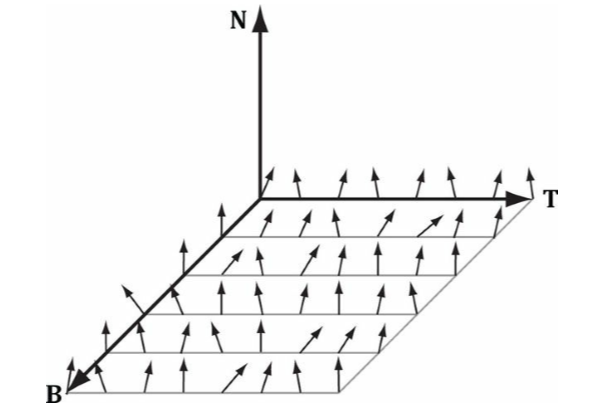
\includegraphics[width=0.8\textwidth]{images/normal_map_tnb.png}
    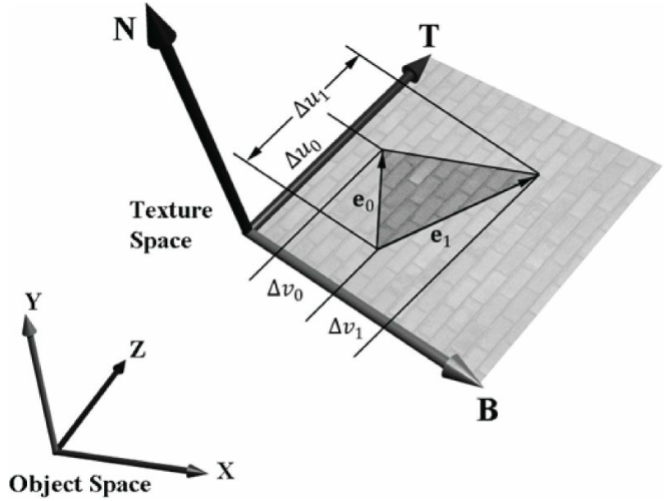
\includegraphics[width=0.8\textwidth]{images/normal_map_tnb_in_object_space.png}
\end{center}
假设三角形的三个顶点为$V_{0},V_{1},V_{2}$,对应的纹理坐标为$(u_{0},v_{0}),(u_{1},v_{1}),(u_{2},v_{2})$
\begin{gather*}
    \because \overrightarrow{e_{0}} = V_{1} - V_{0}, \overrightarrow{e_{1}} = V_{2} - V_{0} \\ 
    \therefore (\Delta u_{0},\Delta v_{0}) = (u_{1} - u_{0}, v_{1} - v{0}),
    (\Delta u_{1}, \Delta v_{1}) = (u_{2} - u_{0}, v_{2} - v_{0}) \\ 
    \therefore \overrightarrow{e_{0}} = \Delta u_{0} \ast \overrightarrow{T} + \Delta v_{0} \ast \overrightarrow{B}, 
    \overrightarrow{e_{1}} = \Delta u_{1} \ast \overrightarrow{T} + \Delta v_{1} \ast \overrightarrow{B} \\    
\end{gather*}
转换为向量表示他们的关系,再转换为矩阵形式,其中逆矩阵等于1除以原矩阵的行列式,再乘以它的伴随矩阵
\begin{gather*}
    \therefore \begin{bmatrix}
        \overrightarrow{e_{0}}.x & \overrightarrow{e_{0}}.y & \overrightarrow{e_{0}}.z \\ 
        \overrightarrow{e_{1}}.x & \overrightarrow{e_{1}}.y & \overrightarrow{e_{1}}.z  
    \end{bmatrix} = \begin{bmatrix}
        \Delta u_{0} & \Delta v_{0} \\ 
        \Delta u_{1} & \Delta v_{1}
    \end{bmatrix} \begin{bmatrix}
        \overrightarrow{T}.x & \overrightarrow{T}.y & \overrightarrow{T}.z \\ 
        \overrightarrow{B}.x & \overrightarrow{B}.y & \overrightarrow{B}.z  
    \end{bmatrix} \\ 
    \begin{bmatrix}
        \overrightarrow{T}.x & \overrightarrow{T}.y & \overrightarrow{T}.z \\ 
        \overrightarrow{B}.x & \overrightarrow{B}.y & \overrightarrow{B}.z  
    \end{bmatrix} = \begin{bmatrix}
        \Delta u_{0} & \Delta v_{0} \\ 
        \Delta u_{1} & \Delta v_{1}
    \end{bmatrix}^{-1} \begin{bmatrix}
        \overrightarrow{e_{0}}.x & \overrightarrow{e_{0}}.y & \overrightarrow{e_{0}}.z \\ 
        \overrightarrow{e_{1}}.x & \overrightarrow{e_{1}}.y & \overrightarrow{e_{1}}.z  
    \end{bmatrix} \\ 
    \because  \begin{bmatrix}
        \Delta u_{0} & \Delta v_{0} \\ 
        \Delta u_{1} & \Delta v_{1}
    \end{bmatrix}^{-1} = \frac{1}{\Delta u_{0} \Delta v_{1} - \Delta v_{0} \Delta u_{1}} \begin{bmatrix}
        \Delta v_{1} & -\Delta v_{0} \\ 
        -\Delta u_{1} & \Delta u_{0}
    \end{bmatrix} \\ 
    \therefore \begin{bmatrix}
        \overrightarrow{T}.x & \overrightarrow{T}.y & \overrightarrow{T}.z \\ 
        \overrightarrow{B}.x & \overrightarrow{B}.y & \overrightarrow{B}.z  
    \end{bmatrix} = \frac{1}{\Delta u_{0} \Delta v_{1} - \Delta v_{0} \Delta u_{1}} \begin{bmatrix}
        \Delta v_{1} & -\Delta v_{0} \\ 
        -\Delta u_{1} & \Delta u_{0}
    \end{bmatrix} \begin{bmatrix}
        \overrightarrow{e_{0}}.x & \overrightarrow{e_{0}}.y & \overrightarrow{e_{0}}.z \\ 
        \overrightarrow{e_{1}}.x & \overrightarrow{e_{1}}.y & \overrightarrow{e_{1}}.z  
    \end{bmatrix} 
\end{gather*}
根据以上公式就可以得到切线T和副法线B。这样就可以在vs中传入normal和tangent,并计算得到binormal,并把这三个向量
标准归一化后传给fs,构造TBN矩阵后乘以从bump map中拿到的法线相乘就是世界坐标的法线了,就可以直接参与光照计算了,
这样的思路是符合光照计算的,思路也清晰。

\par
另一种方法就是把所有的计算都放在切线空间中,这需要把光线向量ray和视图向量view转换到切线空间中,转换的公式是
\begin{gather*}
    \frac{view}{ray} \times TBN^{-1}
\end{gather*}
TBN矩阵的逆矩阵就是转置矩阵,因为构造TBN的都是标准归一化的正交矩阵,这种方法效率更高,因为$\frac{view}{ray}$
在vs中进行转换即可,相比在fs中进行凹凸贴图法线要进行逐像素的转换相比,效率高很多。